\documentclass[conference,a4paper]{IEEEtran}

% Escritura mejorada de fórmulas matemáticas
\usepackage{amsmath}

% Inserción de gráficos
\usepackage{graphicx}

% Escritura de pseudocódigo
\usepackage[kw]{pseudo}

% Escritura mejorada de tablas
\usepackage{booktabs}

% Escritura mejorada de citas bibliográficas
\usepackage{cite}

% Para cambiar el tamaño de la fuente
\usepackage{relsize}

% Macros traducidas
\def\contentsname{Índice general}
\def\listfigurename{Índice de figuras}
\def\listtablename{Índice de tablas}
\def\refname{Referencias}
\def\indexname{Índice alfabético}
\def\figurename{Fig.}
\def\tablename{TABLA}
\def\partname{Parte}
\def\appendixname{Apéndice}
\def\abstractname{Resumen}
% IEEE specific names
\def\IEEEkeywordsname{Palabras clave}
\def\IEEEproofname{Demostración}


\begin{document}

\title{Comparación de Algoritmos de Aprendizaje por Refuerzo en la Navegación de Robots Móviles: Q-Learning, Montecarlo y SARSA}

\author{
  \IEEEauthorblockN{David Fuentelsaz Rodríguez}
  \IEEEauthorblockA{
    \textit{Dpto. Ciencias de la Computación e Inteligencia Artificial}\\
    \textit{Universidad de Sevilla}\\
    Sevilla, España\\
    davfuerod@alum.us.es}
  
  \and
  
  \IEEEauthorblockN{Nombre y apellidos alumno 2}
  \IEEEauthorblockA{
    \textit{Dpto. Ciencias de la Computación e Inteligencia Artificial}\\
    \textit{Universidad de Sevilla}\\
    Sevilla, España\\
    Correos electrónicos UVUS y de contacto (si distinto)}
}

\maketitle


% Resumen
\begin{abstract}
  El objetivo principal de este trabajo es comparar tres algoritmos de aprendizaje por refuerzo: Q-Learning, Montecarlo y SARSA,
  en el contexto de la planificación de rutas para un robot móvil en un entorno con obstáculos. El estudio se centra en evaluar la eficiencia computacional, la convergencia y la robustez
  de cada algoritmo al navegar hacia un destino minimizando la posibilidad de colisión.

  Los resultados obtenidos muestran que cada algoritmo presenta ventajas y desventajas específicas en diferentes aspectos del problema planteado. 
  Q-Learning demostró una rápida convergencia en la mayoría de los escenarios, mientras que Montecarlo ofreció una mejor exploración del espacio de estados. SARSA, por su parte, destacó en entornos altamente estocásticos debido a su enfoque de aprendizaje on-policy. Estas conclusiones ofrecen una guía para la selección del algoritmo más adecuado según las características del entorno y los requisitos del sistema.
\end{abstract}


% Palabras claves
\begin{IEEEkeywords}
  Inteligencia Artificial, Aprendizaje por Refuerzo, Q-Learning, Montecarlo, SARSA, Procesos de Decisión de Markov, Entornos Estocásticos,
  Política, Exploración y Explotación.
\end{IEEEkeywords}


\section{Introducción}

El aprendizaje por refuerzo es un tipo de aprendizaje automático que se enfoca en la toma de decisiones en entornos dinámicos y no deterministas. 
En este tipo de aprendizaje, el agente interactúa con el entorno y recibe recompensas o penalizaciones en función de sus acciones.
El objetivo es maximizar las recompensas y minimizar las penalizaciones para encontrar la política óptima.

Esta técnica tiene una gran variedad de aplicaciones entre las que se encuentran predicciones financieras, robótica, 
videojuegos, medicina o cualquier problema de optimización~\cite{b2}~\cite{b3}.

En el contexto de nuestro trabajo, nos centraremos en la aplicación del aprendizaje por refuerzo a la planificación de rutas para robots móviles. En este problema, un robot con ruedas debe encontrar una ruta segura y eficiente en un entorno con obstáculos. Aunque este problema puede parecer simple a primera vista, la presencia de obstáculos, la estocasticidad en el efecto de las acciones 
y la necesidad de optimizar la ruta para minimizar el tiempo y los recursos hacen que sea un desafío significativo.

Para evaluar la eficacia de los algoritmos de aprendizaje por refuerzo en este contexto, diseñamos tres mapas diferentes que varían en tamaño y porcentaje de obstáculos. Estos mapas nos permitirán comparar y analizar el rendimiento de los algoritmos en una variedad de escenarios.
Comenzamos nuestro trabajo con el mapa de ejemplo proporcionado en la propuesta del trabajo, que tiene dimensiones de 15x51. 

\begin{figure}[h]
  \centering
  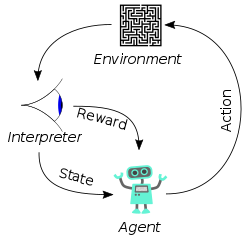
\includegraphics{Reinforcement_learning_diagram.png}
  \caption{Esquema del funcionamiento del aprendizaje por refuerzo.}
  \label{fig:Reinforcement_learning_diagram}
\end{figure}


\section{Preliminares}

En esta sección, proporcionamos una introducción a los conceptos fundamentales del aprendizaje por refuerzo y la planificación de rutas de robots 
móviles en entornos con obstáculos, así como una descripción de los algoritmos de aprendizaje por refuerzo que utilizaremos en nuestro trabajo.

\subsection{Conceptos clave del aprendizaje por refuerzo}

El aprendizaje por refuerzo (RL) es un tipo de aprendizaje automático que entrena al software para tomar decisiones y maximizar una recompensa en un entorno dado. 
Los componentes principales de un sistema de aprendizaje por refuerzo son:

\begin{itemize}
  \item \textbf{Agente}: Es la parte del sistema que toma decisiones e interactúa con el entorno. En nuestro caso, el agente es el robot móvil que busca planificar rutas en un entorno con obstáculos.
  \item \textbf{Entorno}: Es el espacio en el que el agente se mueve y interactúa. En nuestro caso, el entorno es un mapa con obstáculos.
  \item \textbf{Acción}: Una acción es la decisión tomada por el agente en un estado particular. En nuestro caso, tenemos tenemos ocho acciones que representan cada uno de los posibles movimientos que puede efectuar el robot y una 
    acción que representa que el agente permanezca en el mismo estado tras realizarla.
  \item \textbf{Recompensa}: La recompensa es la retroalimentación que el agente recibe del entorno después de tomar una acción en un estado dado. La recompensa puede ser positiva, neutra o negativa (esto sería una penalización).
  \item \textbf{Política}: La política es la estrategia utilizada por el agente para seleccionar acciones en función de los estados del entorno. 
  \item \textbf{Exploración}: Es el proceso de probar nuevas acciones y recopilar información sobre el entorno. La exploración es esencial para que el agente descubra nuevas oportunidades y estrategias que podrían llevar a recompensas a largo plazo más altas.
  \item \textbf{Explotación}: Es el proceso de utilizar la información aprendida para tomar decisiones que maximicen la recompensa inmediata. La explotación es importante para que el agente obtenga la mayor recompensa posible en el momento presente.
\end{itemize}


\subsection{Descripción de los algoritmos}

A continuación, describimos los algoritmos de aprendizaje por refuerzo que utilizados en nuestro trabajo:\newline

\subsubsection{\textbf{Q-Learning}}
El algoritmo Q-Learning es un método de aprendizaje por refuerzo basado en valores que se utiliza para encontrar la política óptima de selección de acciones en un entorno determinado.
Este algoritmo es una variante del aprendizaje por refuerzo que utiliza una función de valor, denominada función Q, para determinar la mejor acción en cada estado del entorno.
No requiere un modelo del entorno y puede manejar problemas con transiciones estocásticas y recompensas sin requerir adaptaciones~\cite{b5}.

El agente explora el entorno y actualiza la tabla Q utilizando la ecuación de Bellman modificada:
\[
Q(s, a) \leftarrow Q(s, a) + \alpha [R(s, a) + \gamma \max_{a'} Q(s', a') - Q(s,a)]
\]
Donde:
\begin{itemize}
    \item \(\alpha\) es el factor de aprendizaje.
    \item \(R(s, a)\) es la recompensa inmediata por tomar la acción \(a\) en el estado \(s\).
    \item \(\gamma\) es el factor de descuento.
    \item \(s'\) es el estado siguiente al tomar la acción \(a\) en el estado \(s\).
    \item \(\max_{a'} Q(s', a')\) es el valor máximo esperado para cualquier acción posible en el estado \(s'\).\newline
\end{itemize}

Se trata de un algoritmo con un enfoque \textit{off-policy}, lo que significa que aprende la función de valor óptima independientemente de la política que el agente esté siguiendo en el momento. Q-Learning actualiza la estimación de la función Q utilizando la recompensa inmediata y el valor máximo de la función Q para el siguiente estado y acción.\newline

\textbf{Hiperparámetros en Q-Learning}
\begin{itemize}
  \item \textbf{Tasa de aprendizaje (\(\alpha\)):} Controla cuánto se actualiza la función Q con nuevas experiencias. Un valor alto de \(\alpha\) permite un aprendizaje rápido pero puede causar oscilaciones, mientras que un valor bajo conduce a un aprendizaje más estable pero más lento.
  \item \textbf{Factor de descuento (\(\gamma\)):} Determina la importancia de las recompensas futuras. Un valor alto de \(\gamma\) hace que el agente valore más las recompensas futuras, lo que es esencial para tareas donde las decisiones tempranas afectan significativamente las recompensas futuras.
  \item \textbf{Estrategia de exploración (\(\epsilon\) en \(\epsilon\)-greedy):} Controla el balance entre exploración y explotación. Un valor alto de \(\epsilon\) fomenta la exploración, lo que es crucial al inicio del aprendizaje, mientras que un valor bajo de \(\epsilon\) fomenta la explotación de acciones conocidas.\newline
\end{itemize}


\subsubsection{\textbf{Montecarlo}}

\subsubsection{\textbf{SARSA}}
El algoritmo SARSA (State-Action-Reward-State-Action) es un algoritmo de aprendizaje por refuerzo que se utiliza para aprender una política óptima en un entorno de Markov discreto. Es bastante similar al algoritmo Q-Learning, 
aunque tiene una serie de diferencias. En primer lugar, SARSA es un algoritmo con un enfoque \textit{on-policy}, lo que significa 
que el agente aprende una política óptima mientras sigue la misma política que está aprendiendo. Este algoritmo también utiliza una tabla Q(s, a) que almacena el valor esperado de tomar la acción a en el estado s. No obstante, 
la forma en la que se actualiza Q presenta una diferencia clave respecto a Q-Learning, como se puede comprobar en la siguiente expresión:

\[
Q(s, a) \leftarrow Q(s, a) + \alpha [R(s, a) + \gamma Q(s', a') - Q(s, a)]
\]

Donde:
\begin{itemize}
    \item \(\alpha\) es el factor de aprendizaje.
    \item \(R(s, a)\) es la recompensa inmediata por tomar la acción \(a\) en el estado \(s\).
    \item \(\gamma\) es el factor de descuento.
    \item \(s'\) es el estado siguiente al tomar la acción \(a\) en el estado \(s\).
    \item \(a'\) es la acción tomada en el estado siguiente \(s'\).\newline
\end{itemize}

En este caso, se puede apreciar que la acción utilizada para actualizar la tabla Q en el siguiente estado es la seleccionada por la política actual. Al seguir un enfoque \textit{on-policy}, SARSA, por lo general, suele ser un algoritmo más lento en la convergencia a la política óptima, especialmente en entornos complejos.\newline

\textbf{Hiperparámetros en SARSA}
\begin{itemize}
  \item \textbf{Tasa de aprendizaje (\(\alpha\)):} Controla cuánto se actualiza la función Q con nuevas experiencias. Un valor alto de \(\alpha\) permite un aprendizaje rápido pero puede causar oscilaciones, mientras que un valor bajo conduce a un aprendizaje más estable pero más lento.
  \item \textbf{Factor de descuento (\(\gamma\)):} Determina la importancia de las recompensas futuras. Un valor alto de \(\gamma\) hace que el agente valore más las recompensas futuras, lo que es esencial para tareas donde las decisiones tempranas afectan significativamente las recompensas futuras.
  \item \textbf{Estrategia de exploración (\(\epsilon\) en \(\epsilon\)-greedy):} Controla el balance entre exploración y explotación. Un valor alto de \(\epsilon\) fomenta la exploración, lo que es crucial al inicio del aprendizaje, mientras que un valor bajo de \(\epsilon\) fomenta la explotación de acciones conocidas.\newline
\end{itemize}

\subsection{Trabajos relacionados}
Para un mejor entendimiento de cómo realizar la implementación de los algoritmos, se han revisado algunos trabajos realizados:
\begin{itemize}
  \item Reinforcement Learning: An Introduction~\cite{b1}.
\end{itemize}

\section{Metodología}

En esta sección, describiremos el método implementado en nuestro trabajo. Abordaremos los siguientes aspectos:

\begin{itemize}
  \item Descripción del entorno de trabajo.
  \item Detalles de la implementación de los algoritmos de aprendizaje por refuerzo (Q-Learning, Montecarlo y SARSA).
  \item Proceso experimental y evaluación de los resultados.
\end{itemize}

\subsection{Descripción del entorno de trabajo}

En el desarrollo de este trabajo, se empleó un entorno de simulación implementado en un Jupyter Notebook. El entorno de simulación se basó en un mapa de ejemplo proporcionado en el trabajo, el cual consiste en una cuadrícula que representa el entorno en el que se moverá el robot móvil. La cuadrícula está compuesta por casillas, algunas de las cuales contienen obstáculos (representadas con unos), mientras que otras están libres de ellos (representadas con ceros).

A partir del mapa de ejemplo, se generaron dos mapas adicionales para aumentar la variabilidad en los escenarios de prueba. Estos mapas proporcionaron diferentes configuraciones de entorno para evaluar el desempeño de los algoritmos de aprendizaje por refuerzo.

Las casillas iniciales y destino fueron seleccionadas aleatoriamente dentro de cada mapa generado, asegurándose de que ninguna de ellas fuera una casilla con obstáculos. Esta selección aleatoria garantizó la variabilidad en los escenarios de prueba y permitió evaluar el desempeño de los algoritmos en diferentes configuraciones del entorno.

En este entorno simulado, el robot móvil parte de una casilla inicial aleatoria y tiene como objetivo llegar a una casilla destino específica. Durante la simulación, el robot puede moverse entre casillas adyacentes en la cuadrícula, siguiendo una política determinada por los algoritmos de aprendizaje por refuerzo implementados. La interacción del robot con el entorno se realiza mediante acciones discretas.

Este enfoque de simulación proporcionó un entorno controlado y reproducible para evaluar el rendimiento de los algoritmos de aprendizaje por refuerzo en la planificación de rutas de robots móviles. Además, permitió explorar diferentes estrategias de navegación y analizar su efectividad en la resolución de problemas de planificación de rutas en entornos con obstáculos.

\begin{figure}[h]
  \centering
  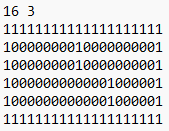
\includegraphics{Ejemplo_mapa.png}
  \caption{Ejemplo mapa generado con la casilla objetivo.}
  \label{fig:Ejemplo_mapa}
\end{figure}

\subsection{Implementación de los algoritmos de aprendizaje por refuerzo}

\textbf{Funciones auxiliares\newline}
Aquí se describen las funciones auxiliares que han sido utilizadas en la implementación de los algoritmos de aprendizaje por refuerzo.\newline

1. Método para leer el mapa de un fichero de texto


\begin{figure}[h]
  \begin{pseudo}*
    \hd{\fn{lee\_mapa}}(\textit{fichero}) \\*
    \multicolumn{2}{l}{\textbf{Entrada}: Nombre del archivo \textit{fichero}} \\*
    \multicolumn{2}{l}{\textbf{Salida}: Matriz que representa el mapa y dimensiones del mapa} \\*
    \multicolumn{2}{l}{\textbf{Algoritmo}:}\\
    Leer las líneas del archivo \textit{fichero} y convertirlas a matriz \\
    Devolver la matriz y sus dimensiones
  \end{pseudo}
  \caption{Pseudocódigo de la función \texttt{lee\_mapa}.}
  \label{fig:lee_mapa}
\end{figure}

2. Método para comprobar si una casilla contiene un obstáculos\newline

\begin{figure}[h]
  \begin{pseudo}*
    \hd{\fn{hay\_colision}}(\textit{estado}) \\*
    \multicolumn{2}{l}{\textbf{Entrada}: Casilla en la que se encuentra el robot \textit{estado}} \\*
    \multicolumn{2}{l}{\textbf{Salida}: Valor booleano que indica si hay colisión} \\*
    \multicolumn{2}{l}{\textbf{Algoritmo}:} \\
    Verificar si hay un obstáculo en \textit{estado} \\
    Devolver \textbf{true} si hay colisión, \textbf{false} en caso contrario
  \end{pseudo}
  \caption{Pseudocódigo del método \texttt{hay\_colision}.}
  \label{fig:hay_colision}
\end{figure}

3. Método para aplicar una acción en un estado

\begin{figure}[h]
  \begin{pseudo}*
    \hd{\fn{aplica\_accion}}(\textit{estado}, \textit{accion}) \\*
    \multicolumn{2}{l}{\textbf{Entrada}: \textit{estado} y \textit{accion}} \\*
    \multicolumn{2}{l}{\textbf{Salida}: Nuevo \textit{estado}} \\*
    \multicolumn{2}{l}{\textbf{Algoritmo}:}\\
    \textbf{Si} hay colisión \textbf{entonces} \\
    \> Devolver \textit{estado} \\
    $x, y \leftarrow$ Coordenadas de \textit{estado} \\
    \textbf{Si} \textit{accion} es norte \textbf{entonces} \\
    \> $y \leftarrow y + 1$ \\
    \textbf{Si no, si} \textit{accion} es sur \textbf{entonces} \\
    \> $y \leftarrow y - 1$ \\
    \textbf{Si no, si} \textit{accion} es este \textbf{entonces} \\
    \> $x \leftarrow x + 1$ \\
    \textbf{Si no, si} \textit{accion} es oeste \textbf{entonces} \\
    \> $x \leftarrow x - 1$ \\
    \textbf{Sino, si} \textit{accion} es noreste \textbf{entonces} \\
    \> $x, y \leftarrow x + 1, y + 1$ \\
    \textbf{Si no, si} \textit{accion} es sureste \textbf{entonces} \\
    \> $x, y \leftarrow x + 1, y - 1$ \\
    \textbf{Si no, si} \textit{accion} es suroeste \textbf{entonces} \\
    \> $x, y \leftarrow x - 1, y - 1$ \\
    \textbf{Si no, si} \textit{accion} es noroeste \textbf{entonces} \\
    \> $x, y \leftarrow x - 1, y + 1$ \\
    Devolver $(x, y)$ como nuevo \textit{estado}
  \end{pseudo}
  \caption{Pseudocódigo de \texttt{aplica\_accion}.}
  \label{fig:aplica_accion}
\end{figure}

4. Método para obtener los estados libres de obstáculos

\begin{figure}[h]
  \begin{pseudo}*
    \hd{\fn{estados\_sin\_obstaculos}}() \\*
    \multicolumn{2}{l}{\textbf{Salida}: Lista de estados sin obstáculos} \\*
    \multicolumn{2}{l}{\textbf{Algoritmo}:}\\
    Inicializar una lista vacía llamada \textit{estados\_sin\_obstaculos} \\
    \fn{Para cada} estado \textit{en} \textit{nav\_estados} \fn{hacer} \\
    \> \fn{Si no} \fn{hay\_colision}(estado) \fn{entonces} \\
    \> \> Agregar el estado a la lista \textit{estados\_sin\_obstaculos} \\
    Devolver la lista \textit{estados\_sin\_obstaculos}
  \end{pseudo}
  \caption{Pseudocódigo detallado de \texttt{estados\_sin\_obstaculos}.}
  \label{fig:estados_sin_obstaculos}
\end{figure}

Siendo \textit{nav\_estados} la variable global con todos los estados del entorno.\newline

5. Método para obtener los posibles desvíos del agente al realizar una acción

\begin{figure}[h]
  \begin{pseudo}*
    \hd{\fn{obtiene\_posibles\_errores}}(\textit{accion}) \\*
    \multicolumn{2}{l}{\textbf{Entrada}: \textit{accion}} \\*
    \multicolumn{2}{l}{\textbf{Salida}: Lista de posibles acciones erróneas} \\*
    \multicolumn{2}{l}{\textbf{Algoritmo}:}\\
    \textbf{Si} \textit{accion} es norte \textbf{entonces} \\
    \> \textit{errores} $\leftarrow$ ['NE', 'NO'] \\
    \textbf{Si no, si} \textit{accion} es sur \textbf{entonces} \\
    \> \textit{errores} $\leftarrow$ ['SE', 'SO'] \\
    \textbf{Si no, si} \textit{accion} es este \textbf{entonces} \\
    \> \textit{errores} $\leftarrow$ ['NE', 'SE'] \\
    \textbf{Si no, si} \textit{accion} es oeste \textbf{entonces} \\
    \> \textit{errores} $\leftarrow$ ['NO', 'SO'] \\
    \textbf{Si no, si} \textit{accion} es noreste \textbf{entonces} \\
    \> \textit{errores} $\leftarrow$ ['N', 'E'] \\
    \textbf{Si no, si} \textit{accion} es noroeste \textbf{entonces} \\
    \> \textit{errores} $\leftarrow$ ['N', 'O'] \\
    \textbf{Si no, si} \textit{accion} es sureste \textbf{entonces} \\
    \> \textit{errores} $\leftarrow$ ['S', 'E'] \\
    \textbf{Si no, si} \textit{accion} es suroeste \textbf{entonces} \\
    \> \textit{errores} $\leftarrow$ ['S', 'O'] \\
    \textbf{Si no} \\
    \> \textit{errores} $\leftarrow$ [] \\
    Devolver \textit{errores}
  \end{pseudo}
  \caption{Pseudocódigo de \texttt{obtiene\_posibles\_errores}.}
  \label{fig:obtiene_posibles_errores}
\end{figure}


6. Método para escoger una acción a partir de la política \(\epsilon-greedy\)\
  
\begin{figure}[h]
  \begin{pseudo}*
    \hd{\fn{escoger\_accion}}(\textit{estado}, \textit{epsilon}) \\*
    \multicolumn{2}{l}{\textbf{Entrada}: Estado \textit{estado} y valor de epsilon \textit{epsilon}} \\*
    \multicolumn{2}{l}{\textbf{Salida}: Acción seleccionada} \\*
    \multicolumn{2}{l}{\textbf{Algoritmo}:}\\
    \textbf{Si} \textit{estado} no está en la tabla Q \textbf{entonces} \\
    \> Inicializar los valores de \textit{estado} a cero en la tabla Q \\
    \\
    \textbf{Si} un número aleatorio entre 0 y 1 es menor que \textit{epsilon}\\
    \> \textbf{Seleccionar} una acción aleatoria de entre todas las posibles \\
    \textbf{Si no} \\
    \> \textbf{Seleccionar} la mejor acción conocida \\
    \\
    Devolver la acción seleccionada
  \end{pseudo}
  \caption{Pseudocódigo de \texttt{escoger\_accion}.}
  \label{fig:escoger_accion}
\end{figure}

7. Método para obtener la política a partir de los valores de la tabla Q\newline\newline\newline\newline\newline\newline\newline\newline

\begin{figure}[h]
  \begin{pseudo}*
    \hd{\fn{obtener\_politica}}(\textit{Q}) \\*
    \multicolumn{2}{l}{\textbf{Entrada}: Tabla \textit{Q}} \\*
    \multicolumn{2}{l}{\textbf{Salida}: Política basada en \textit{Q}} \\*
    \multicolumn{2}{l}{\textbf{Algoritmo}:} \\
    Inicializar \textit{politica} como diccionario vacío \\
    \textbf{Para cada} estado \textit{en} nav\_estados \textbf{hacer} \\
    \> \textbf{Si} estado \textit{está en} Q\_table \textbf{entonces} \\
    \> \> \textit{politica[estado]} $\leftarrow$ índice de max(\textit{Q\_table[estado]}) \\
    \> \textbf{Sino} \\
    \> \> \textit{politica[estado]} $\leftarrow$ 0 \\
    \textbf{Retornar} \textit{politica}
  \end{pseudo}
  \caption{Pseudocódigo de la función \texttt{obtener\_politica}.}
  \label{fig:obtener_politica}
\end{figure}

8. Método para obtener la recompensa de aplicar una acción a un estado

\begin{figure}[h]
  \begin{pseudo}*
    \hd{\fn{obtiene\_recompensa}}(\textit{estado}, \textit{accion}) \\*
    \multicolumn{2}{l}{\textbf{Entrada}: Estado actual \textit{estado}, acción a tomar \textit{accion}} \\*
    \multicolumn{2}{l}{\textbf{Salida}: Recompensa correspondiente} \\*
    \multicolumn{2}{l}{\textbf{Algoritmo}:} \\
    \textit{x, y} $\leftarrow$ \textit{estado} \\
    \textbf{Si} \textit{estado} es igual a \textit{destino} \textbf{entonces} \\
    \> devolver \textit{recompensa\_objetivo\_alcanzado} \\
    \textbf{Si} hay colisión en \textit{estado} \textbf{entonces} \\
    \> devolver -\textit{penalizacion\_colision} \\
    \textbf{Si} \textit{accion} es igual a 'esperar' \textbf{entonces} \\
    \> devolver -\textit{penalizacion\_esperar} \\
    \textbf{Para cada} \textit{accion\_error} \\ en obtiene\_posibles\_errores(\textit{accion}) \textbf{hacer} \\
    \> \textit{estado\_vecino} $\leftarrow$ aplica\_accion(\textit{estado}, \textit{accion\_error}) \\
    \> \textbf{Si} hay colisión en \textit{estado\_vecino} \textbf{entonces} \\
    \> \> devolver -\textit{penalizacion\_casilla\_adyacente\_obstaculo} \\
  \end{pseudo}
  \caption{Pseudocódigo de la función \texttt{obtiene\_recompensa}.}
  \label{fig:obtiene_recompensa}
\end{figure}

En este caso, \textit{recompensa\_objetivo\_alcanzado}, \textit{penalizacion\_colision}, \textit{penalizacion\_esperar} y \textit{penalizacion\_casilla\_adyacente\_obstaculo}
son variables globales que se usan en el método para definir el valor de la recompensa en diferentes situaciones.\newline

Tras presentar todas las funciones auxiliares utilizadas en la implementación de los algoritmos, procedemos a detallar la implementación de Q-Learning, Montecarlo y SARSA.\newline 

\textbf{Q-Learning\newline}

En primer lugar nos encontramos con el algoritmo de Q-Learning.

\begin{figure}[h]
  \begin{pseudo}
    \textbf{Q-Learning}: \\
    Inicializar $Q$ como diccionario vacío \\
    Parámetros: $\alpha = 0.2$, $\gamma = 0.9$, $\epsilon = 0.3$, \\ $epocas = 5000$, $max\_pasos = 100$ \\
    Para cada época: \\
    \> Estado aleatorio sin obstáculos \\
    \> Para cada paso: \\
    \> \textit{accion\_index} $\leftarrow$ escoger\_accion(\textit{estado}, $\epsilon$) \\
    \> \textit{accion} $\leftarrow$ nav\_acciones[\textit{accion\_index}] \\
    \> Aplicar acción, obtener nuevo estado y recompensa \\
    Si \textit{estado} \textnormal{no está en} \textit{Q\_table} entonces \\+
      Inicializar \textit{Q\_table}[\textit{estado}] con ceros \\-
    \textbf{Fin Si} \\
    Si \textit{nuevo\_estado} \textnormal{no está en} \textit{Q\_table} entonces \\+
      Inicializar \textit{Q\_table}[\textit{nuevo\_estado}] con ceros \\-
    \textbf{Fin Si} \\
    \textit{mejor\_accion\_nueva} $\leftarrow$ máximo de \textit{Q\_table}[\textit{nuevo\_estado}] \\
    \textit{Q\_table}[\textit{estado}][\textit{accion}] $\leftarrow$ \textit{Q\_table}[\textit{estado}][\textit{accion}] + \\
    \> \textit{alpha} * (\textit{recompensa} + \textit{gamma} * \textit{mejor\_accion\_nueva} - \\
    \> \textit{Q\_table}[\textit{estado}][\textit{accion}])\\
    \> Si estado destino o terminal, terminar \\
  \end{pseudo}
  \caption{Pseudocódigo del algoritmo Q-Learning.}
  \label{fig:q-learning}
\end{figure}



\begin{thebibliography}{00}
\bibitem{b1} Richard S. Sutton y Andrew G. Barto. Reinforcement Learning: An Introduction.
MIT Press, 2018.
\bibitem{b2} https://www.codificandobits.com/curso/aprendizaje-por-refuerzo-nivel-basico/2-ejemplos-reales-aplicacion-aprendizaje-por-refuerzo/
\bibitem{b3} https://www.aprendemachinelearning.com/aprendizaje-por-refuerzo/
\bibitem{b4} K. Elissa, ``Title of paper if known,'' unpublished.
\bibitem{b5} https://es.wikipedia.org/wiki/Q-learning
\bibitem{b6} Y. Yorozu, M. Hirano, K. Oka, and Y. Tagawa, ``Electron spectroscopy studies on magneto-optical media and plastic substrate interface,'' IEEE Transl. J. Magn. Japan, vol. 2, pp. 740--741, August 1987 [Digests 9th Annual Conf. Magnetics Japan, p. 301, 1982].
\bibitem{b7} M. Young, The Technical Writer's Handbook. Mill Valley, CA: University Science, 1989.
\end{thebibliography}


\end{document}
